
%%%%%%%%%%%%%%%%%%%%%%%%%%%%%%%%%%%%%%%%%%%%%%%%%%%%%%%%%%%%%%%%%%%%%%%%%%%%%%%%%%%%%%%
%%%%%%%%%%%%%%%%%%%%%%%%%%%%%%%%%%%%%%%%%%%%%%%%%%%%%%%%%%%%%%%%%%%%%%%%%%%%%%%%%%%%%%%
% 
% This top part of the document is called the 'preamble'.  Modify it with caution!
%
% The real document starts below where it says 'The main document starts here'.

\documentclass[12pt]{article}

\usepackage{amssymb,amsmath,amsthm}
\usepackage[top=1in, bottom=1in, left=1.25in, right=1.25in]{geometry}
\usepackage{fancyhdr}
\usepackage{enumerate}
\usepackage{listings}
\usepackage{graphicx}
\usepackage{float}

\usepackage{mwe}
\usepackage{caption}
\usepackage{subcaption}
% Comment the following line to use TeX's default font of Computer Modern.
\usepackage{times,txfonts}



\makeatletter
\renewcommand*\env@matrix[1][*\c@MaxMatrixCols c]{%
  \hskip -\arraycolsep
  \let\@ifnextchar\new@ifnextchar
  \array{#1}}
\makeatother

\newtheoremstyle{homework}% name of the style to be used
  {18pt}% measure of space to leave above the theorem. E.g.: 3pt
  {12pt}% measure of space to leave below the theorem. E.g.: 3pt
  {}% name of font to use in the body of the theorem
  {}% measure of space to indent
  {\bfseries}% name of head font
  {:}% punctuation between head and body
  {2ex}% space after theorem head; " " = normal interword space
  {}% Manually specify head
\theoremstyle{homework} 

% Set up an Exercise environment and a Solution label.
\newtheorem*{exercisecore}{Exercise \@currentlabel}
\newenvironment{exercise}[1]
{\def\@currentlabel{#1}\exercisecore}
{\endexercisecore}

\newcommand{\localhead}[1]{\par\smallskip\noindent\textbf{#1}\nobreak\\}%
\newcommand\solution{\localhead{Solution:}}

%%%%%%%%%%%%%%%%%%%%%%%%%%%%%%%%%%%%%%%%%%%%%%%%%%%%%%%%%%%%%%%%%%%%%%%%
%
% Stuff for getting the name/document date/title across the header
\makeatletter
\RequirePackage{fancyhdr}
\pagestyle{fancy}
\fancyfoot[C]{\ifnum \value{page} > 1\relax\thepage\fi}
\fancyhead[L]{\ifx\@doclabel\@empty\else\@doclabel\fi}
\fancyhead[C]{\ifx\@docdate\@empty\else\@docdate\fi}
\fancyhead[R]{\ifx\@docauthor\@empty\else\@docauthor\fi}
\headheight 15pt

\def\doclabel#1{\gdef\@doclabel{#1}}
\doclabel{Use {\tt\textbackslash doclabel\{MY LABEL\}}.}
\def\docdate#1{\gdef\@docdate{#1}}
\docdate{Use {\tt\textbackslash docdate\{MY DATE\}}.}
\def\docauthor#1{\gdef\@docauthor{#1}}
\docauthor{Use {\tt\textbackslash docauthor\{MY NAME\}}.}
\makeatother

% Shortcuts for blackboard bold number sets (reals, integers, etc.)
\newcommand{\Reals}{\ensuremath{\mathbb R}}
\newcommand{\Nats}{\ensuremath{\mathbb N}}
\newcommand{\Ints}{\ensuremath{\mathbb Z}}
\newcommand{\Rats}{\ensuremath{\mathbb Q}}
\newcommand{\Cplx}{\ensuremath{\mathbb C}}
%% Some equivalents that some people may prefer.
\let\RR\Reals
\let\NN\Nats
\let\II\Ints
\let\CC\Cplx
%%%%%%%%%%%%%%%%%%%%%%%%%%%%%%%%%%%%%%%%%%%%%%%%%%%%%%%%%%%%%%%%%%%%%%%%%%%%%%%%%%%%%%%
%%%%%%%%%%%%%%%%%%%%%%%%%%%%%%%%%%%%%%%%%%%%%%%%%%%%%%%%%%%%%%%%%%%%%%%%%%%%%%%%%%%%%%%
% 
% The main document start here.

% The following commands set up the material that appears in the header.
\doclabel{Stat 461: Homework 3}
\docauthor{Stefano Fochesatto}
\docdate{February 5, 2022}

\begin{document}

\begin{exercise}{1} Consider the following data, 
  \begin{footnotesize}
  \begin{verbatim}
    group1 <- structure(c(16, 11, 14, 20, 13, 12, 13, 21, 11, 15, 16, 11,
    14, 20, 13, 12, 13, 21, 11, 15, 28, 27, 27, 23, 26, 25, 26, 35, 21, 
    26, 26, 29, 27, 24, 29, 23, 22, 22, 16, 23, 54, 50, 36, 41, 51, 
    49, 39, 48, 44, 44, 54, 50, 36, 41, 51, 49, 39, 48, 44, 44), .Dim = c(20L, 
    3L), .Dimnames = list(NULL, c("G1", "H1", "J1")))
    #
    group2 <- structure(c(21, 11, 16, 19, 15, 22, 16, 19, 19, 18, 21,
    11, 16, 19, 15, 22, 16, 19, 19, 18, 30, 33, 35, 23, 32, 37, 31, 24, 21, 
    28, 24, 20, 31, 38, 24, 28, 19, 30, 25, 33, 44, 45, 30, 29, 38, 
    47, 35, 44, 50, 35, 44, 45, 30, 29, 38, 47, 35, 44, 50, 35), 
    .Dim = c(20L, 3L), .Dimnames = list(NULL, c("G2", "H2", "J2")))
    #
    group1; group2
  \end{verbatim}
  \end{footnotesize}

  \begin{enumerate}
    \item[a] What are the null and alternative hypotheses?  What are the assumptions of Hotelling's T2 test?\\
    \solution  The null hypothesis of Hotelling's T2 test assumes that the means of the two groups are equal, the alternative 
    hypothesis says that they are different,
    \begin{equation*}
      H_0: \mu_1 = \mu_2,
    \end{equation*}
    \begin{equation*}
      H_a: \mu_1 \neq \mu_2.
    \end{equation*}
    Hotelling's T2 test assumes that the groups are sampled from a multivariate normal distribution, the samples in each group are independent, and the two groups have 
    the same covariance matrix.  
    \vspace{.15in}

    \item[b] Use any functions you wish to perform a Hotelling's T2 test (0.05 significance level) on the data in group1 and group2.\\
    \solution Using the HotellingsT2() function from the ICSNP package we get the following,\\
    \textbf{Code:}
      \begin{center}
      \lstinputlisting[basicstyle = \footnotesize]{r1.txt}
      \end{center}
    With a p-value of 0.001498 we would reject the null hypothesis and say that at a $\alpha = .05$ significance level there is a difference between the 
    means of the two groups. 
    \vspace{.15in}



    \item[c] Perform a t-test on each of the three variables and a graphic of your choice. What are your conclusions?  Assume the 0.05 significance level.\\
    \solution We can perform a t-test on each of the variables in the groups using t.test(). Doing so we find that both the J and G variable are significantly different 
    with p-values around .006. The H variable had a p-value of 0.05312 which would fail to reject the null at the $\alpha = .05$ level, but it is close enough that accross the whole 
    group we could likely say that our findings with the individual t-tests match our Hotelling's T2.\\
      \textbf{Code:}
        \begin{center}
        \lstinputlisting[basicstyle = \footnotesize]{r2.txt}
        \end{center}
      \begin{figure}[H]
        \begin{center}
          \caption{Scatterplot Matrix of the 2 groups. black is group1, red is group2.}
        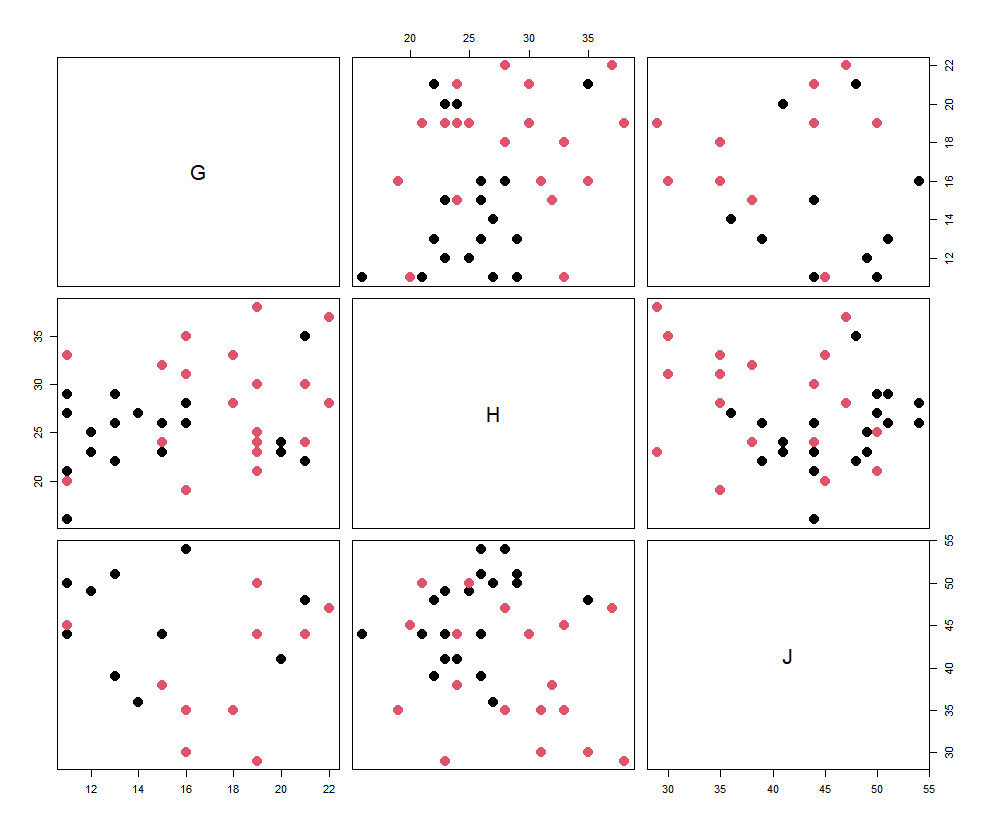
\includegraphics[width = \textwidth]{Rplot09.png}
        \end{center}
      \end{figure}







    \vspace{.15in} 
    
    \item[d] Use a Box's M test (you can use the function in biotools, or any other one in R you wish to use) to test... something.  
    What IS it's null and alternative hypothesis?  What is your conclusion?  Discuss how this influences your analysis.  Assume the 0.05 significance level.\\
    \solution  Box's M test is a diagnostic test to check the assumption of equal covariance matrices among the groups. The null hypothesis assumes that the covariance matrices 
    are equal and the alternative hypothsis assumes that they are not. Wrangling the data to use the boxM() function from biotools we get a p-value of .3079, therefore at the 
    $\alpha = 0.05$ significance level we would fail to reject the null hypothesis and conclude that the covariance matrices for these groups are the same.\\
    \textbf{Code:}
      \begin{center}
      \lstinputlisting[basicstyle = \footnotesize]{r3.txt}
      \end{center}
    \vspace{.15in}









    \item[e] What IS a significance level?\\
    \solution A significance can be described as a measure of type I error for hypotheses test. 
    To recall type I error is when we reject the null when it is the truth. A $\alpha = .05$ significance level means 
    that we are accepting a five percent chance of committing a type I error.  We compare this $\alpha$ value to the p-value of a test statistic
    because the p-value is the probability of obtaining out test-statistic under the null hypothesis. Clearly when the p-value is zero we must reject the 
    null, this doesn't always happen so we accept a certain level of uncertainty so when p-values come out lower than our significance level we also reject the null. 
  \end{enumerate}  
\end{exercise}
\vspace{1in}




\begin{exercise}{2} 
  Skim the article (on Blackboard):\\
  WJ Cooper, MW Westneat (2009)  Form and function of damselfish skulls:  rapid and repeated evolution into a limited number of trophic niches.  BMC Evolutionary Biology 9 (24).
  Among a variety of univariate and multivariate tests, they perform a MANOVA.  What are they testing?  What are the conclusions?  Do they follow this with simpler tests?  If so, which ones?\\
  \solution The goal of the paper was to use morphological and biomechanical analysis to see if there was a significant difference in the anatomical structure among different species of damselfish
  mainly grouped together as omnivores, herbivores, and planktivores. The tests described in the results section are used to see if there is a significant difference in the anatomical data among these groups of 
  damselfish. Using the Wilk's Lambda and Goodall's F test they found that there was indeed a significant difference in the anatomy of these different groups of damselfish. A pairwise ANOVA found that the majority 
  of the difference came from the planktivore group, as the pairwise test between omnivores and herbivores failed to reject the null with a p-value of .1977. 
  The paper also mentions further pairwise analysis comparing the individual predictors in each group, stating that of the seven that where found to be significant, the planktivore group was considered in six of them. 
  This further analysis was documented in additional file 4, which was not accessible through the link in the document.  

\end{exercise}
\vspace{1in}



\begin{exercise}{3}
  \begin{enumerate}
    \item[a] In Appendix One I run a MANOVA followed by two ANOVAs, one for the first variable (over all three groups) and one for a second variable. Interpret the output. Is the result obvious from the plotted data?\\
    \solution The MANOVA using the Wilk's Lambda test statistic finds that on the $\alpha = .05$ significance level there is a significant difference in the means of each group. The further ANOVAs test each individaul variable 
    for each group. We find that means of the second variable were the most distinguishable, with a p-value of .05473 as apposed to the first variable's .16. Looking at the plot I would say that this result is not obvious, maybe there is a slight  
     clustering which is pushing the means of each group apart, but at a first glance it is not clear to me that the means of each group are significantly different. Even more so the results of the individual ANOVA are not obvious from looking at the plot. 
     Maybe after knowing the results of the tests one could distinguish the difference between the means along the y-axis but without prior knowledge I wouldn't make that conclusion.    
    \vspace{.15in}
    
    


    \item[b] I could also conduct three Hotelling's T2 test, one for each pair of groups. What would this tell me? The output is in Appendix Two.\\   
    \solution Running pairwise Hotelling's T2 tests tells you which means among your groups are significantly different. The pairwise analysis found that group2 and group3 showed 
    the most significant difference, with a p-value of .02993, while all other test failed to reject the null at a $\alpha = .05$ significance level. 

  \end{enumerate}
\end{exercise}
\vspace{1in}





\begin{exercise}{4} We want to model growth curves for two responses, y1 and y2.  
We'll do that by regressing on $x1$ (1,2,3,...,20), $x2 = x1^2$, and $x3 = x1^3$.
  \begin{footnotesize}
    \begin{verbatim}
      Y <- structure(c(1958, 1922, 2004, 1924, 1903, 1950, 1864, 1952, 
      1979, 1954, 1977, 1976, 1938, 2005, 2027, 1932, 2025, 2084, 2082, 
      2065, 1035, 987, 971, 966, 908, 881, 928, 999, 941, 944, 931, 898, 
      918, 971, 966, 998, 989, 993, 1060, 1030), .Dim = c(20L, 2L), .Dimnames = list(
          NULL, c("y1", "y2")))
      #
      X <- structure(c(-9, -8, -7, -6, -5, -4, -3, -2, -1, 0, 1, 2, 3, 4, 
      5, 6, 7, 8, 9, 10, 81, 64, 49, 36, 25, 16, 9, 4, 1, 0, 1, 4, 
      9, 16, 25, 36, 49, 64, 81, 100, -729, -512, -343, -216, -125, 
      -64, -27, -8, -1, 0, 1, 8, 27, 64, 125, 216, 343, 512, 729, 1000
      ), .Dim = c(20L, 3L), .Dimnames = list(NULL, c("x1", "x2", "x3"
      )))
      #
      cbind(X,Y)
    \end{verbatim}
  \end{footnotesize}

\begin{enumerate}
  \item[a] Perform (using any function you wish in R) 
  a multiple linear regression to predict $y1$ from $x1,x2,x3$, 
  then another one predicting $y2$ from $x1,x2,x3$.  
  Write down the slopes and intercepts.\\
  \solution  Performing the two MLRs using the lm() command we get the following summary report, \\
      \textbf{Code:}
        \begin{center}
        \lstinputlisting[basicstyle = \footnotesize]{r4.txt}
        \end{center}
  




  
  \vspace{.15in}

  \item[b] Run the functions lm(Y~X), 
  and then Anova() on the output of the lm(Y~X) function.  
  What does this tell you?\\
  \solution Running the full multivariate model we get a summary report which combines the previous individual MLR summary reports. This is as expected given 
  the analogous nature of the multivariate model. Running the Anova() function(I ran Anova() from the car package instead of anova()) we get the Pillai test statistic, which 
  with a p-value of $0.0003634$ we reject the null and conclude that there is a significant difference among the response means.\\
    \textbf{Code:}
    \begin{center}
    \lstinputlisting[basicstyle = \footnotesize]{r5.txt}
    \end{center}
  \vspace{.15in}


  \item[c]  Finally, run the following matrix equation, 
  and check to see if you get the coefficients from both regressions (from a) in one run:
  \begin{footnotesize}
    \begin{verbatim}
      X <- cbind(rep(1,20),X)  #adding a column of ones, for the intercept
      B <- solve(t(X)%*%X)%*%t(X)%*%Y
    \end{verbatim}
  \end{footnotesize}
  \solution Running the given matrix equation we do get the dame values from a, and b.\\
  \textbf{Code:}
  \begin{center}
  \lstinputlisting[basicstyle = \footnotesize]{r6.txt}
  \end{center}













\end{enumerate}








  
\end{exercise}
















\end{document}


















